\section{Analysis and results}
Firstly we have to build a business model canvas for Meta social media
platforms. They all more or less use the same principles and offer the
same experience to their customers, what changes between them is the
actual content published and the target demographic for the platform.
A version could be the picture \ref{fig:fbcanvas}.

\begin{figure}
  \centering
  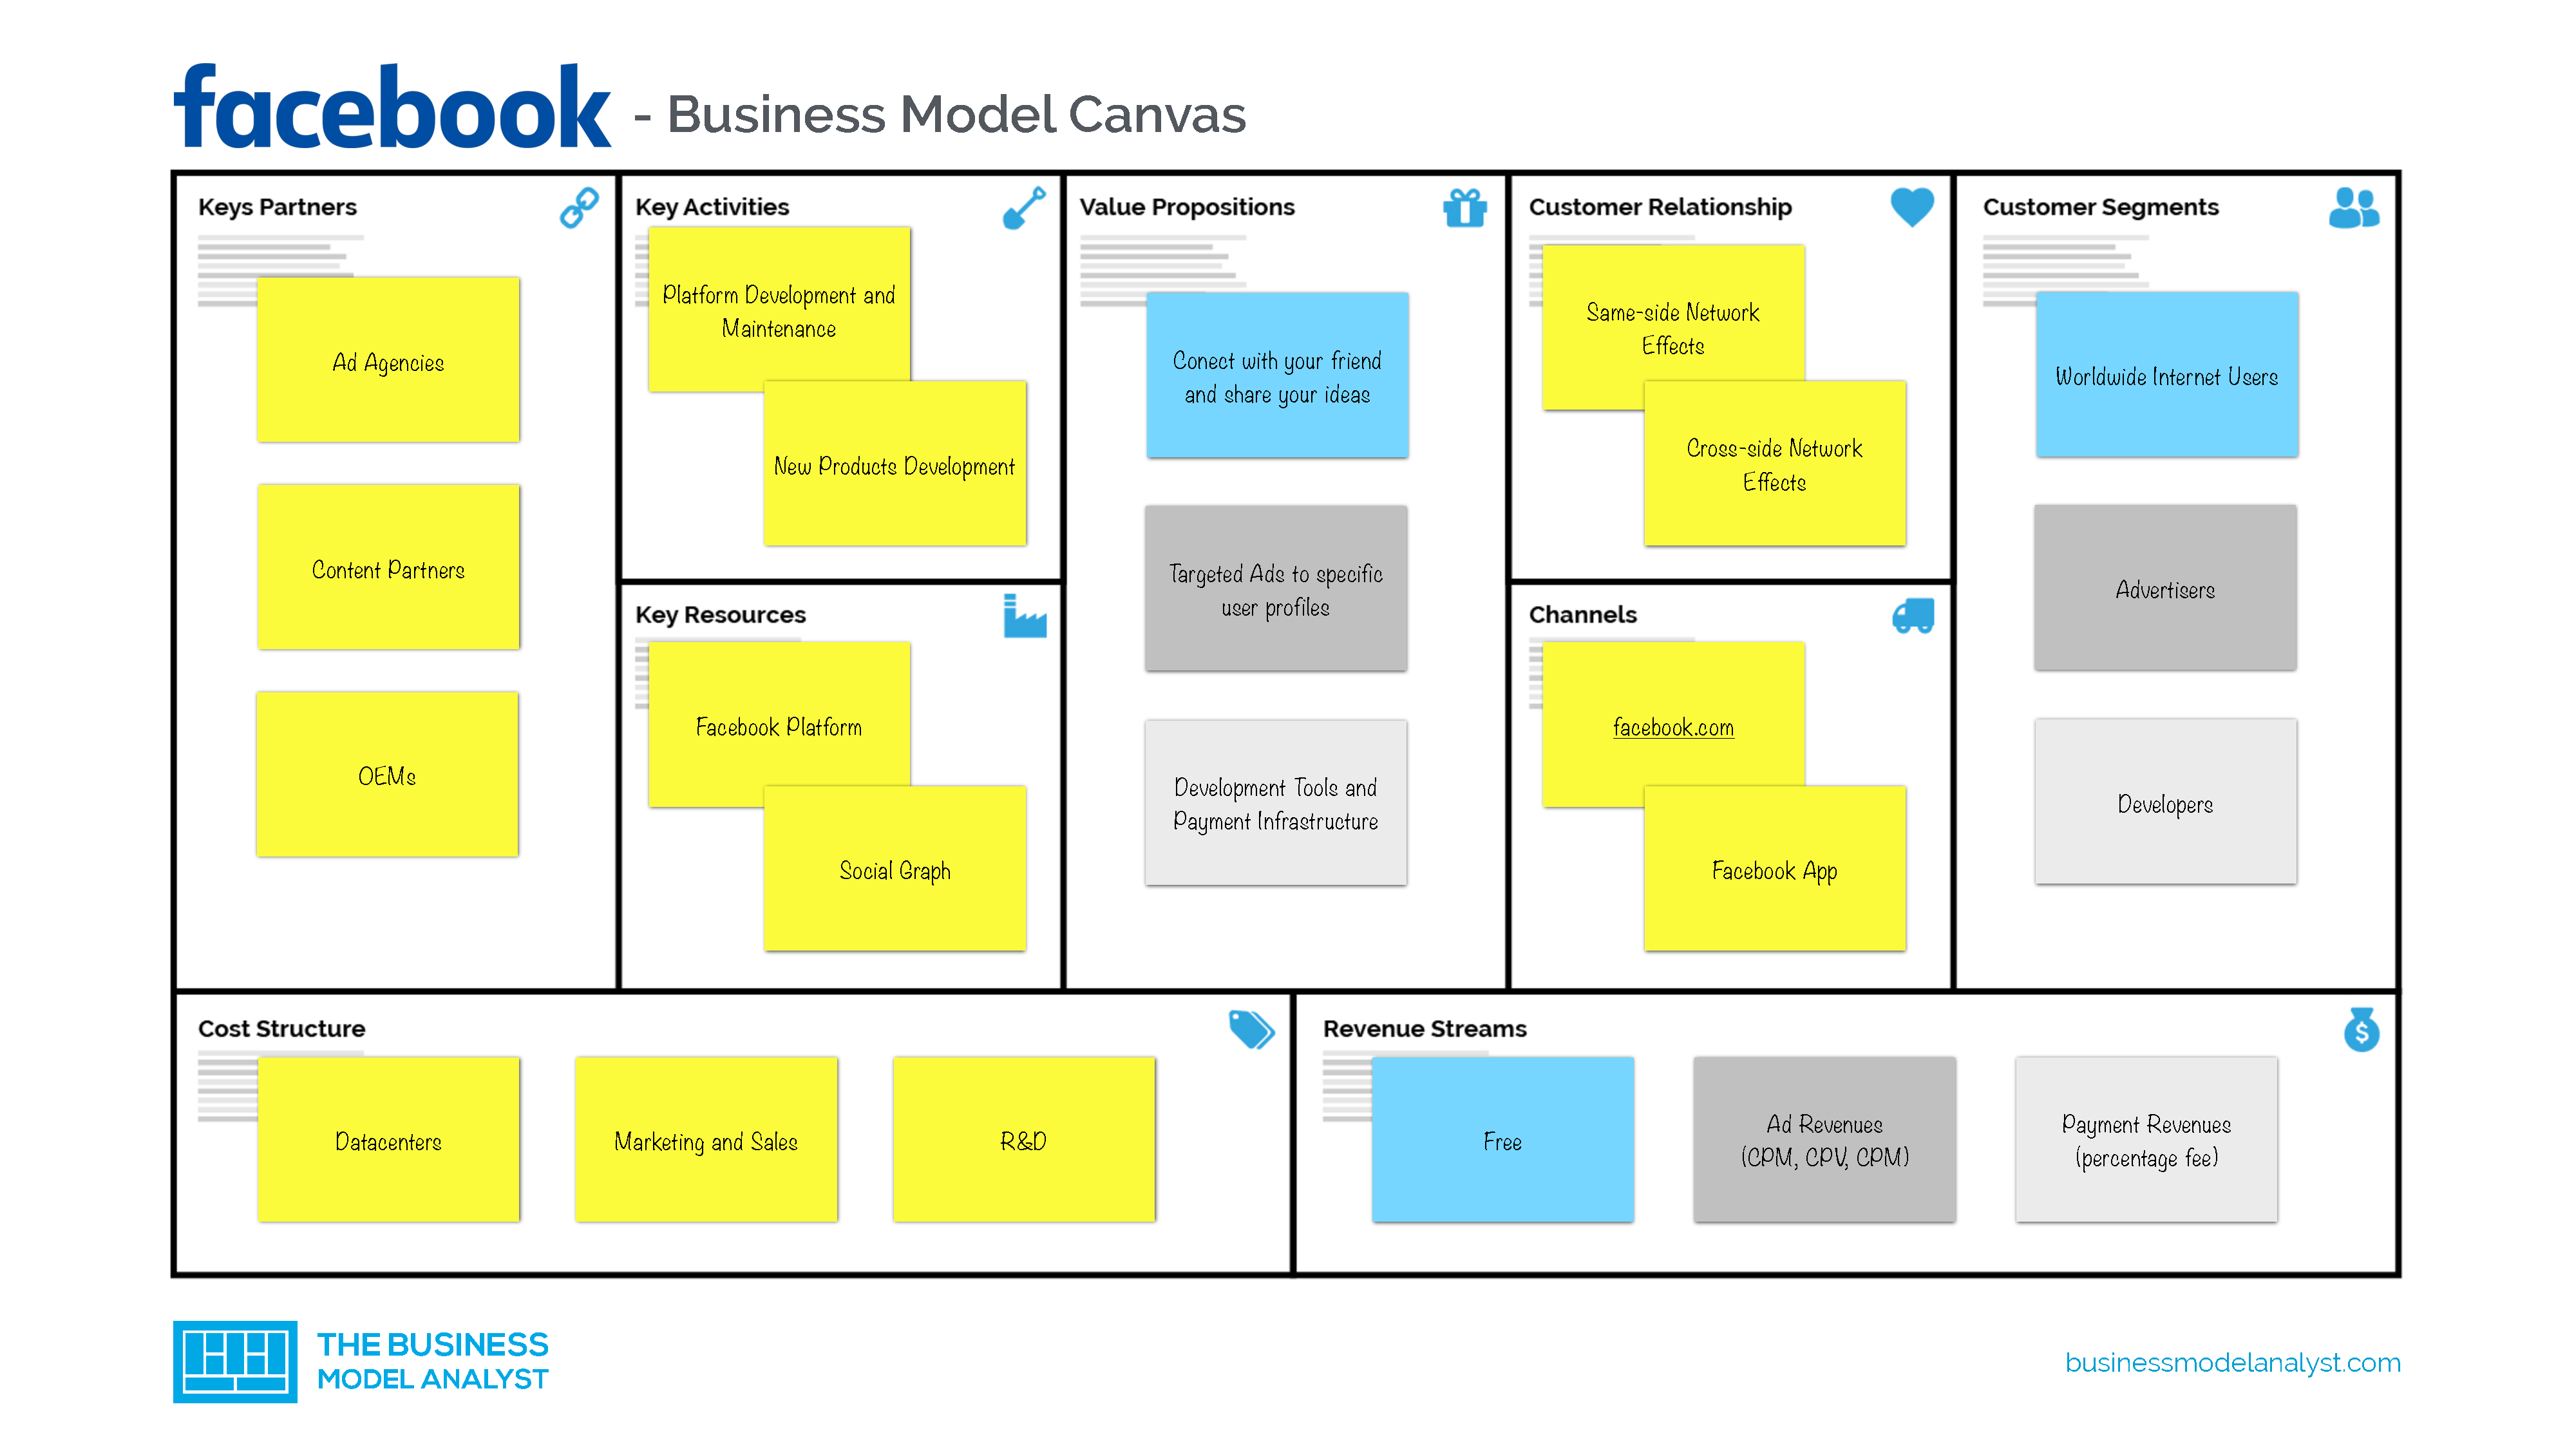
\includegraphics[width=\textwidth]{images/fbcanvas.pdf}
  \caption{Meta social media business model canvas, source: \cite{site:analyst}}
  \label{fig:fbcanvas}
\end{figure}

The model was build on the social network facebook, one of the two
main social platforms along with instagram owned by Meta. The model
however works also for instagram, since the core business of the two
platforms is the same. The main point of this canvas is that there are
three main customers of Meta's platforms. Users, who use the platform
for free, and provide no direct revenue stream for the company. These
customers however are essential to the platforms, since they rapresent
the real value that is later sold to the other two clients. This means
that is vital to the platform to mantain a good overall relashionship
with its users. In this scenario a problem has emerged in the last
decade. From \cite{art:fortuna2018survey} we can see how the
recognition of hate speech has become more and more a problem that
social platform had to face in the last years, and how more and more
literature has been published about it. Meta, with its two main
products Instagram and Facebook is no exception. This particular
phenomena becomes a problem when the backbone AI of the platform is
trained in order to maximize angagment, and for some users, hate
speech is the content that keeps them inside of Meta's social
platforms. But hate speech is controversial, and nor advertisers, nor
some users want to see it. For the company has become more and more of
a problem that of investors and users opting out of the platform for
this very reason.

Here starts the journey of another AI trained to remove hate speech
from the platform. Over the years the platform has used various
approach to model the different systems to tackle hate speech, and
recently a new model composed by few-shot-learners has emerged. The
main problem is that these systems have to evolve rapidly, since the
laguage is doing so naturally. Traditional systems evolve thanks to
new data in a matter of months, but few-shot-learners require less
time, and the method developed by Meta requires even less time,
outperforming other comparabel FSLs up to 55\%, and 12\% in averge
\cite[pp.~5-8]{art:entailing}.

In the business model we presented, this innovation regards users and
advertisers. Users to create a better social community inside of the
platform, discouraging disengagement due to hate speech, advertisers
since generally these customers dont like teir products associated to
hate speech.

\begin{figure}
  \centering
  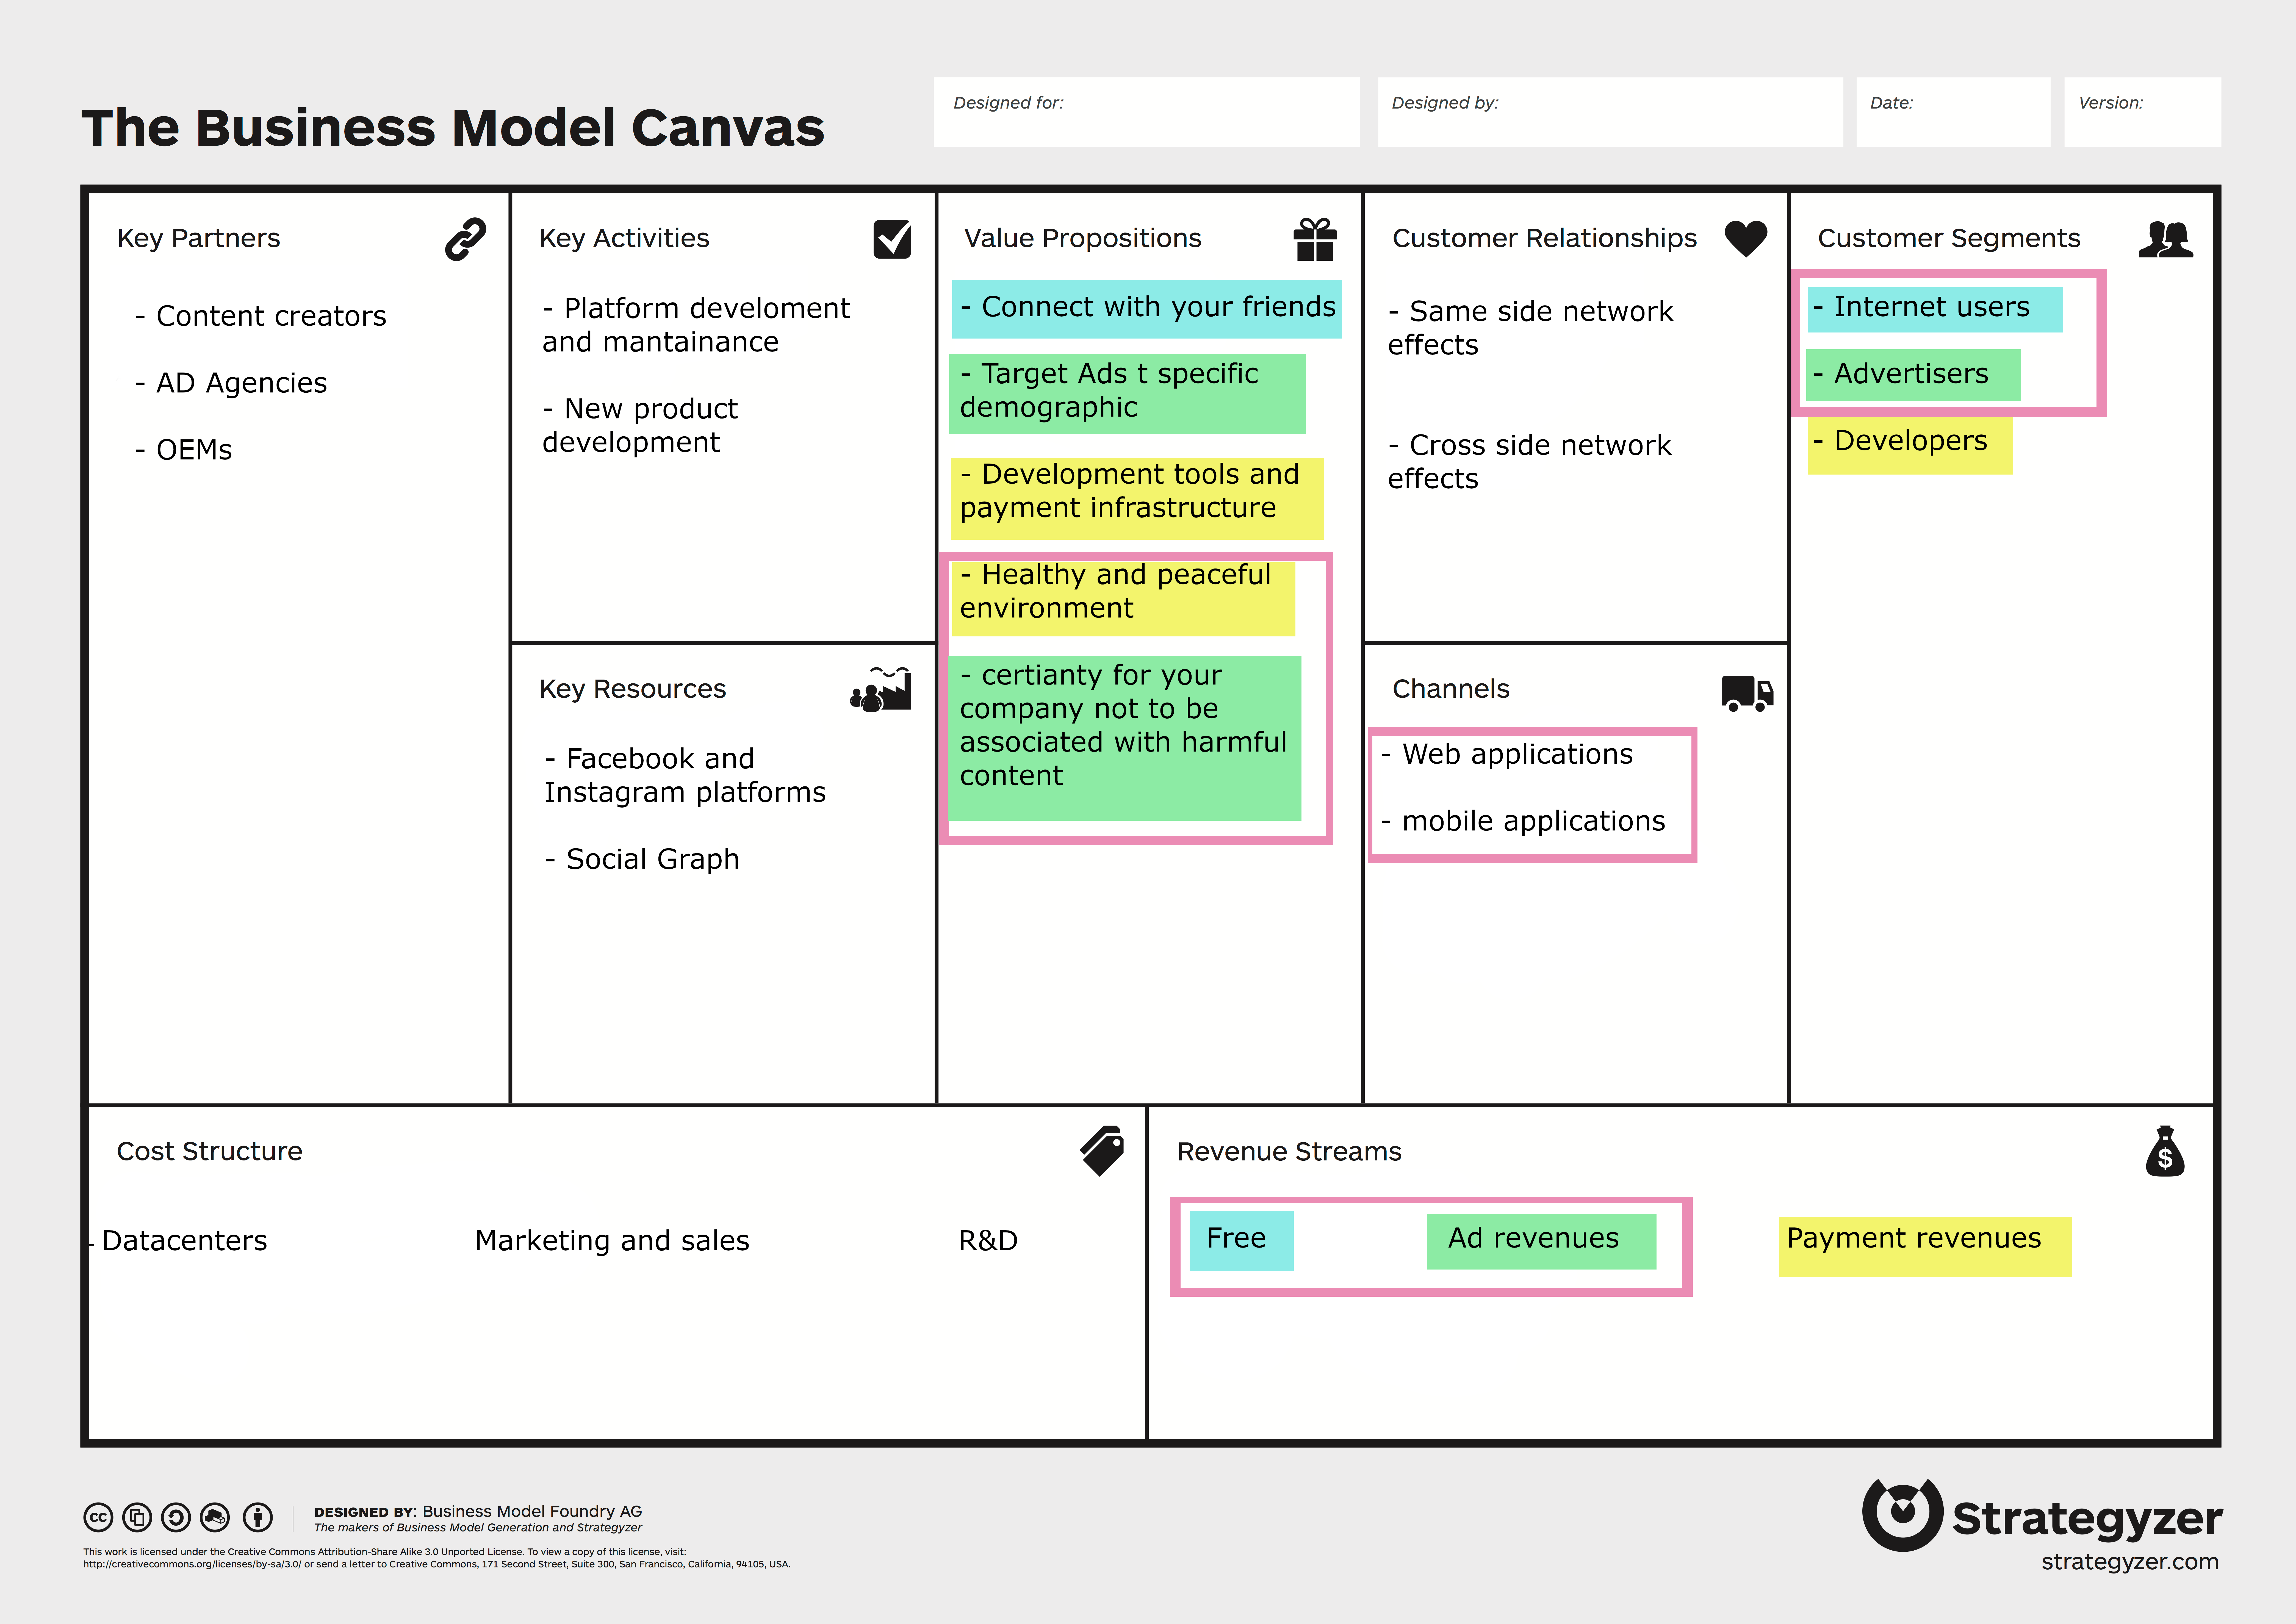
\includegraphics[width=.8\textwidth]{images/newcanvas}
  \caption{new value propositions in the business model due to
    innovations in the AI recognising hate speech, source: author own
    elaoration.}
  \label{fig:newcanvas}
\end{figure}

In red in the figure \ref{fig:newcanvas} we can see what targets and
channels the innovation tackles, along with what new value proposition
it offers to users and advertisers.
